\documentclass[compress]{beamer}
\usepackage{ifthen,verbatim}

\newcommand{\isnote}{}
\xdefinecolor{lightyellow}{rgb}{1.,1.,0.25}
\xdefinecolor{darkblue}{rgb}{0.1,0.1,0.7}

%% Uncomment this to get annotations
%% \def\notes{\addtocounter{page}{-1}
%%            \renewcommand{\isnote}{*}
%% 	   \beamertemplateshadingbackground{lightyellow}{white}
%%            \begin{frame}
%%            \frametitle{Notes for the previous page (page \insertpagenumber)}
%%            \itemize}
%% \def\endnotes{\enditemize
%% 	      \end{frame}
%%               \beamertemplateshadingbackground{white}{white}
%%               \renewcommand{\isnote}{}}

%% Uncomment this to not get annotations
\def\notes{\comment}
\def\endnotes{\endcomment}

\setbeamertemplate{navigation symbols}{}
\setbeamertemplate{headline}{\mbox{ } \hfill
\begin{minipage}{5.5 cm}
\vspace{-0.75 cm} \small
\end{minipage} \hfill
\begin{minipage}{4.5 cm}
\vspace{-0.75 cm} \small
\begin{flushright}
\ifthenelse{\equal{\insertpagenumber}{1}}{}{Jim Pivarski \hspace{0.2 cm} \insertpagenumber\isnote/\pageref{numpages}}
\end{flushright}
\end{minipage}\mbox{\hspace{0.2 cm}}\includegraphics[height=1 cm]{../cmslogo} \hspace{0.1 cm} \includegraphics[height=1 cm]{../tamulogo} \hspace{0.01 cm} \vspace{-1.05 cm}}

\begin{document}
\begin{frame}
\vfill
\begin{center}
\textcolor{darkblue}{\Large CSC Alignment with Beam-Halo Data}

\vfill
\begin{columns}
\column{0.3\linewidth}
\begin{center}
\large
\textcolor{darkblue}{Jim Pivarski}

\vspace{0.2 cm}
Alexei Safonov
\end{center}

\column{0.3\linewidth}
\begin{center}
\large
K\'aroly Banicz
\end{center}
\end{columns}

\begin{columns}
\column{0.3\linewidth}
\begin{center}
\scriptsize
{\it Texas A\&M University}
\end{center}
\column{0.3\linewidth}
\begin{center}
\scriptsize
{\it US-CMS}
\end{center}
\end{columns}

\vfill
30 September, 2008

\end{center}
\end{frame}

%% \begin{notes}
%% \item This is the annotated version of my talk.
%% \item If you want the version that I am presenting, download the one
%% labeled ``slides'' on Indico (or just ignore these yellow pages).
%% \item The annotated version is provided for extra detail and a written
%% record of comments that I intend to make orally.
%% \item Yellow notes refer to the content on the {\it previous} page.
%% \item All other slides are identical for the two versions.
%% \end{notes}

\begin{frame}
\frametitle{HIP-based program}
\small
\textcolor{darkblue}{\large Long-term (collisions)}
\begin{itemize}
\item Align each chamber with tracker-fitted tracks (baseline MuonHIP)
\begin{itemize}
  \item no coupling between track-fitting and alignment
  \item no hierarchial uncertainties
  \item yields tracker-muon interalignment
\end{itemize}
\item Prefer cosmic rays so that tracks through a given chamber don't all
  come from the same part of the tracker (or use $Z$ mass constraint)
\item Need to be cautious of magnetic field uncertainties, esp.\ in endcap
\end{itemize}

\vfill
\textcolor{darkblue}{\large Medium-term (CRAFT)}
\begin{itemize}
\item Align 200 out of 250 DTs with baseline MuonHIP
\item Align chambers within endcap rings using Overlaps Procedure
\item Align endcap rings to tracker as rigid bodies
\begin{itemize}
\item Plot alignment correction as a function of $q/p_T$ to
  distinguish effects of misalignment (constant), multiple scattering (symmetric, through origin),
  and \mbox{magnetic field (antisymmetric)\hspace{-1 cm}}
\end{itemize}

\end{itemize}
\end{frame}

\begin{frame}
\small
\vspace{0.5 cm}
\textcolor{darkblue}{\large Short-term (now)}
\begin{itemize}
\item Align endcap disks to muon barrel in CRUZET (done)
\item Align chambers in ME$-$2/1 and ME$-$3/1 using Overlaps Procedure (mostly done, debugging)
\item Align disks and wheels to tracker in a large globalMuon sample \\ (if there is a large globalMuon sample)
\end{itemize}

\vspace{0.4 cm}
\hspace{-0.83 cm} \uncover<2>{\textcolor{darkblue}{\Large Overlaps Procedure}}

\vspace{0.1 cm}
\uncover<2>{\begin{itemize}
\item Segments in overlap region of neighboring CSCs must agree on slope and intercept
\item Average difference $\alpha_{i,i+1}$ is a relative correction between $A_i$ and $A_{i+1}$, solve for global solution (at most 36$\times$36 matrix inversion)
\end{itemize}}

\uncover<2>{\begin{columns}
\column{0.18\linewidth}
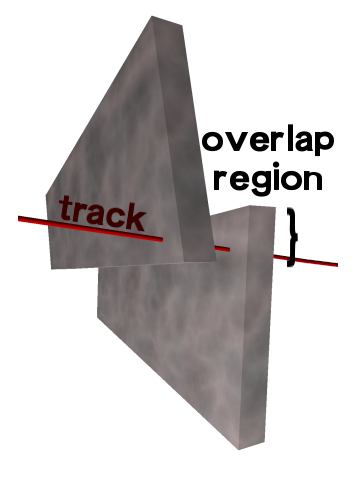
\includegraphics[width=\linewidth]{overlaps.png}
\column{0.7\linewidth}
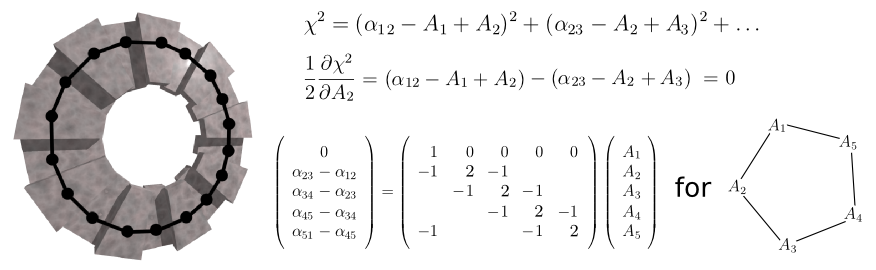
\includegraphics[width=\linewidth]{matrix_description_onestation.png}
\end{columns}}
\end{frame}

\begin{frame}
\frametitle{Important parameters}
\small

\begin{columns}
\column{0.18\linewidth}
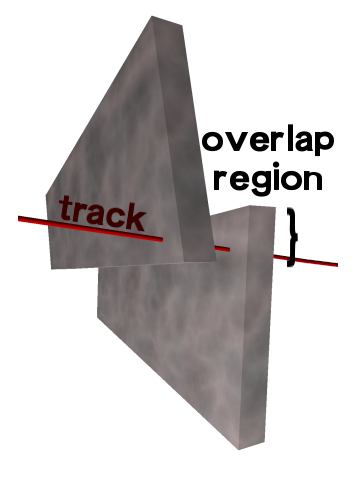
\includegraphics[width=\linewidth]{overlaps.png}
\column{0.25\linewidth}
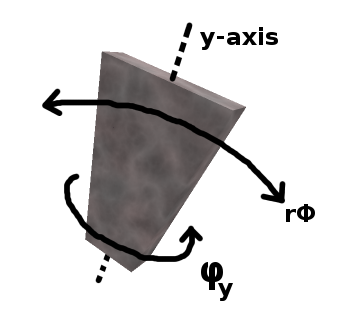
\includegraphics[width=\linewidth]{one_chamber.png}
\column{0.4\linewidth}
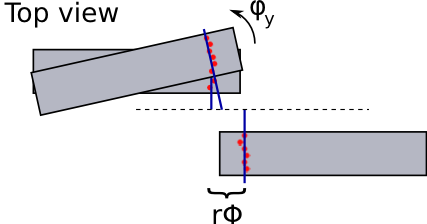
\includegraphics[width=\linewidth]{order_of_parameters.png}
\end{columns}

%% \begin{itemize}
%% \item $\varphi_y$ angles: rotation around axis of symmetry
%% \begin{itemize}
%% \item determined from difference in segment slopes ($d\phi/dz$)
%% \item must be aligned first!
%% \end{itemize}
%% \item $r\phi$ translations: displacement along a circular arc, \mbox{centered on beam\hspace{-1 cm}}
%% \begin{itemize}
%% \item determined from difference in segment intercepts on a common plane between them
%% \end{itemize}
%% \item $\varphi_z$ angles: rotation in plane
%% \begin{itemize}
%% \item determined from intercept difference as a function of $y$
%% \end{itemize}
%% \end{itemize}

\textcolor{darkblue}{$\varphi_y$ angles:} rotation around axis of symmetry
\begin{itemize}
\item determined from difference in segment slopes (1-D linear fit $d\phi/dz$)
\item must be aligned first!
\end{itemize}
\textcolor{darkblue}{$r\phi$ translations:} displacement along a circular arc, \mbox{centered on beamline\hspace{-1 cm}}
\begin{itemize}
\item determined from difference in segment intercepts on a common plane between them
\item local parameters $\Delta x = r\sin(\phi)$, $\Delta y = r(\cos(\phi) - 1)$, $\Delta \varphi_z = \phi$
\end{itemize}
\textcolor{darkblue}{$\varphi_z$ angles:} rotation in plane
\begin{itemize}
\item determined from intercept residual as a function of $y$
\end{itemize}

Apply procedure three times, with appropriate definitions of
$\alpha_{i,i+1}$ and $A_i$ (pedestrian approach is wiser than a
combined fit at this time)
\end{frame}

\begin{frame}
\frametitle{State of software}
\small

\begin{itemize}
\item First draft of procedure was a reparameterization of HIP
\item Final version is very different, very specific to CSC geometry
\item All changes were necessary! (see ``Evolution of Procedure'' backup)
\item This is a correct algorithm: works perfectly in Monte Carlo
\item Encapsulated as a new AlignmentProducer plug-in, to be uploaded to CVS after clean-up
\end{itemize}

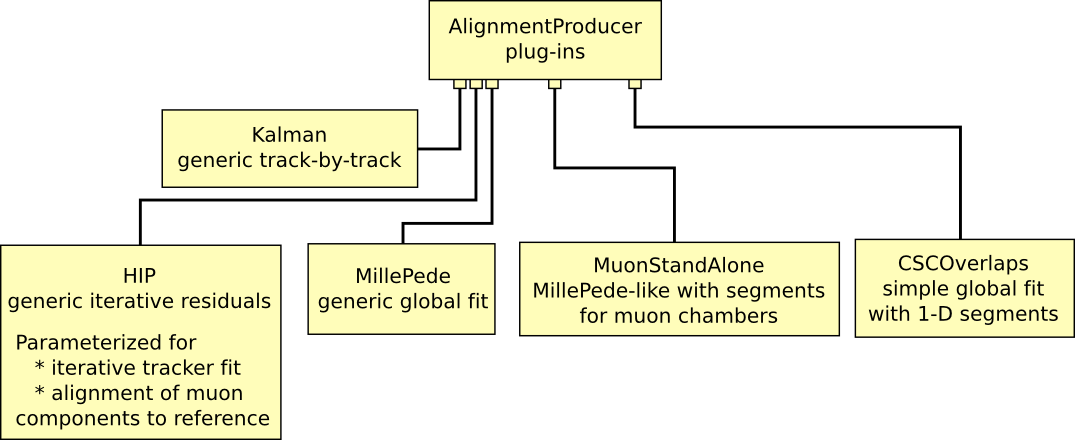
\includegraphics[width=\linewidth]{software.png}
\end{frame}

%% \section*{First section}
%% \begin{frame}
%% \begin{center}
%% \Huge \textcolor{blue}{First section}
%% \end{center}
%% \end{frame}

\begin{frame}
\frametitle{Measuring $\varphi_y$ angles in data}
\small

Three independent methods (for cross-checks):
\begin{columns}
\column{0.6\linewidth}

\begin{enumerate}
\item \textcolor{darkblue}{Overlaps Procedure:} $d\phi/dz$ slope must agree in pairs
\item Generic beam-halo: $d\phi/dz$ must agree on a track from ME$-$2/1 to ME$-$3/1
\item $d\phi/dz$ must be on average zero, because beam-halo tracks come from the LHC (absolute, not pairwise)
\end{enumerate}

\column{0.4\linewidth}
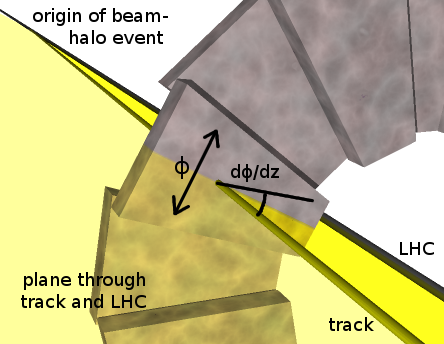
\includegraphics[width=\linewidth]{track_lhc_plane_closeup.png}
\end{columns}

\vspace{-0.2 cm}
\begin{columns}
\column{0.25\linewidth}
\begin{center}
Corrections from \textcolor{darkblue}{(1)} and \textcolor{darkblue}{(3)}:

\vspace{0.3 cm}
\scriptsize Completely different methods, disjoint sets of tracks, reproduces some trends

\end{center}
\column{0.65\linewidth}
\begin{center}
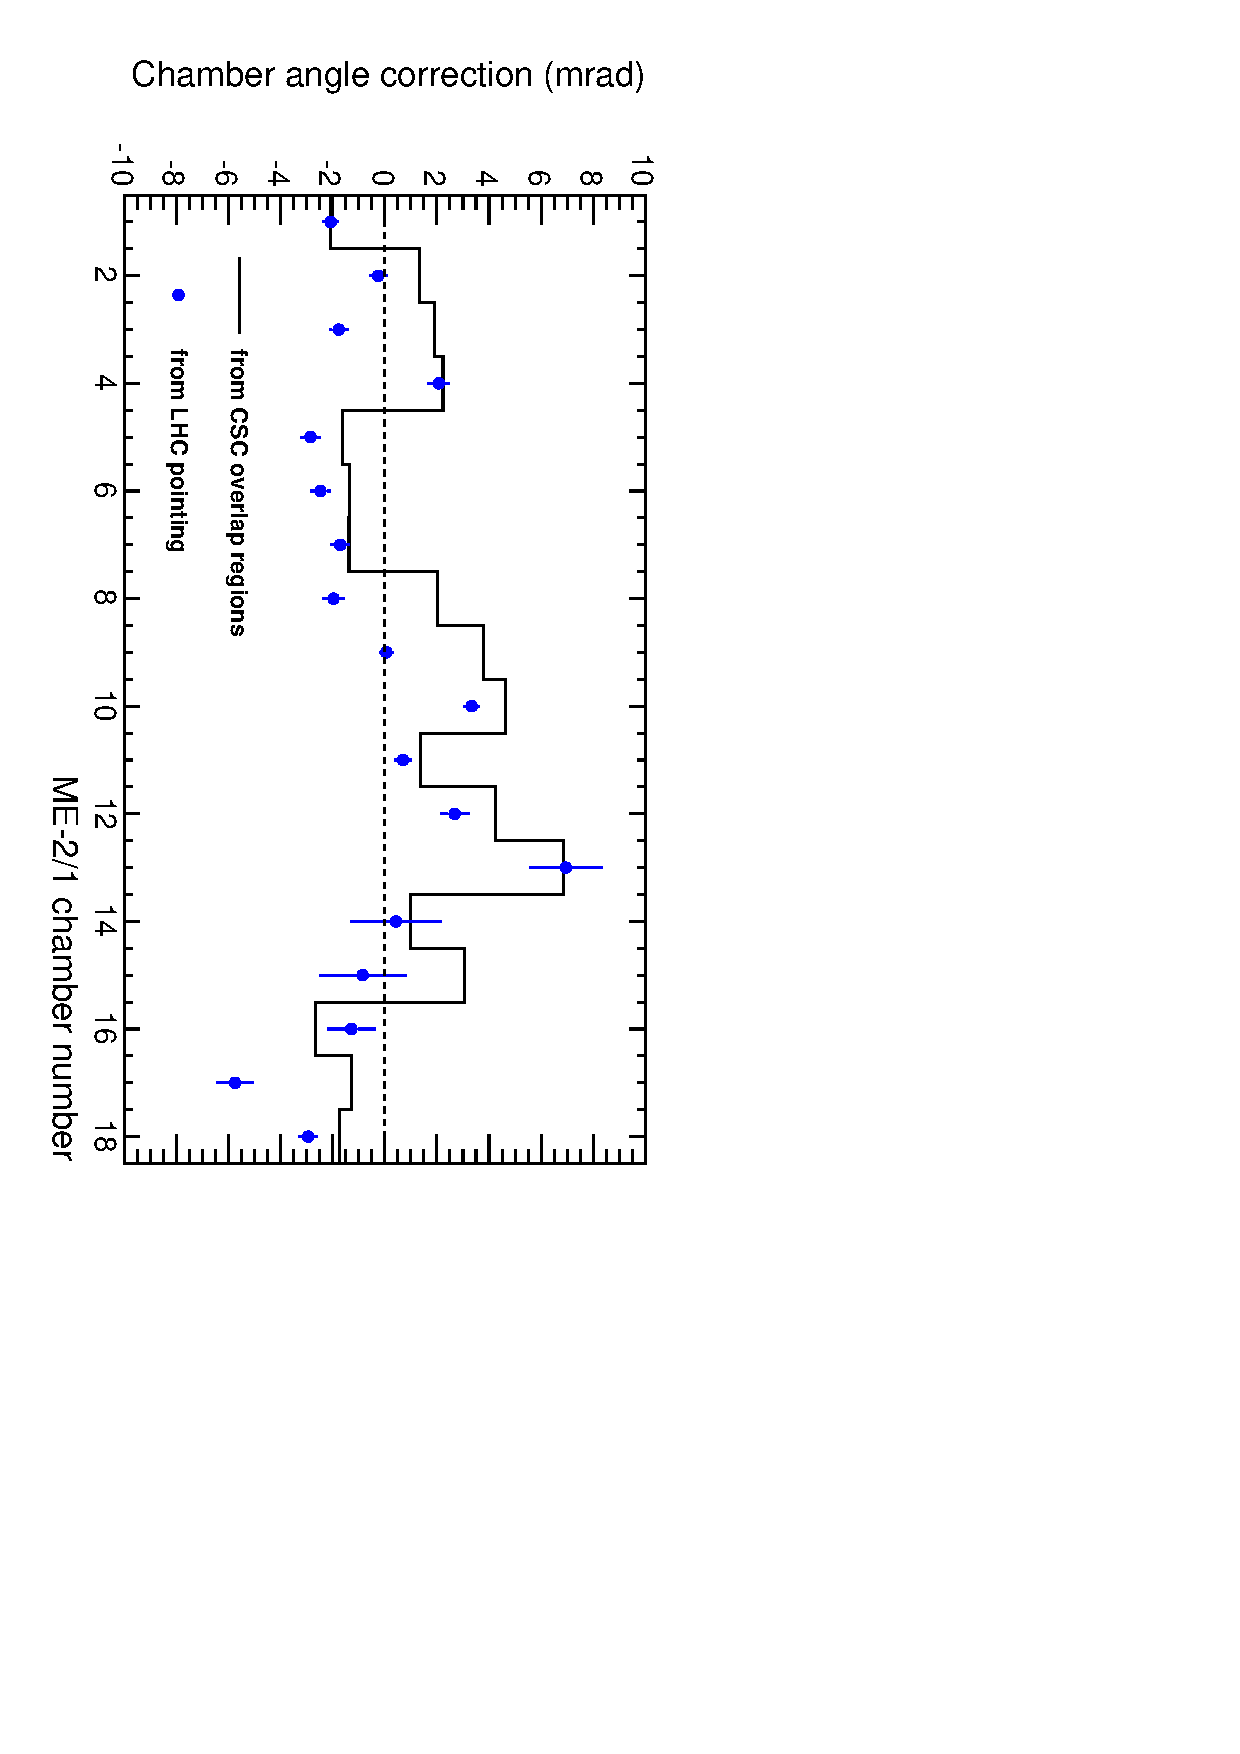
\includegraphics[height=\linewidth, angle=90]{angle_comparison_meminus21.pdf}
\end{center}
\end{columns}
\end{frame}

\begin{frame}
\frametitle{Measuring $r\phi$ positions}
\small

\vspace{0.25 cm}
Taking $\varphi_y$ from LHC pointing for now, attempt $r\phi$ alignment

\vspace{0.5 cm}
\begin{columns}
\column{0.4\linewidth}
Two independent methods:
\begin{enumerate}
\item \textcolor{darkblue}{Overlaps:} track intercepts must match between $N$ and $N+1$
\item Straight-through: track must match between $N_{ME-2/1}$ and $N_{ME-3/1}$
\end{enumerate}

\column{0.65\linewidth}
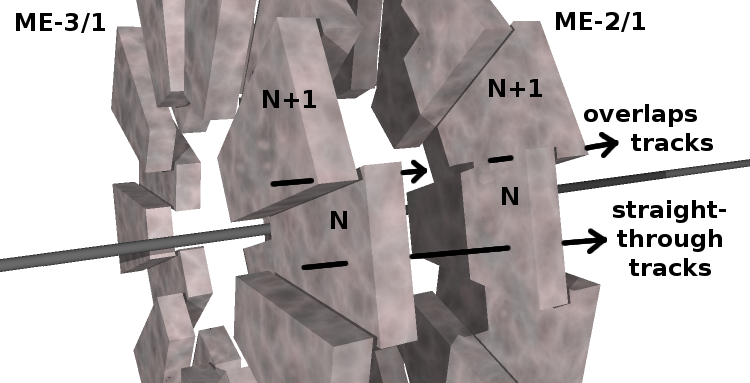
\includegraphics[width=\linewidth]{overlaps_straight_through.png}
\end{columns}

\vspace{0.5 cm}
Align with \textcolor{darkblue}{(1)} and look at a plot of \textcolor{darkblue}{(2)} for each $N$

(data-driven estimate of alignment quality)

\begin{center}
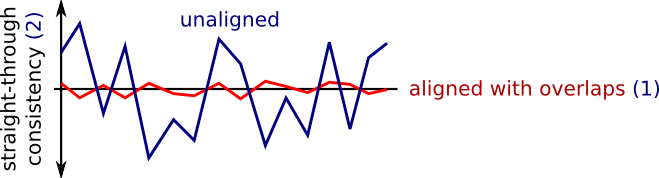
\includegraphics[width=0.7\linewidth]{what_to_expect.png}
\end{center}
\end{frame}

\begin{frame}
\frametitle{Cross-checking $r\phi$ positions}
\small

\only<1>{\begin{itemize}
\item As we apply corrections, we improve alignment (as seen by straight-through tracks) in chambers 1--12 \& 18
\item Chambers 13--16 are unreliable due to poor statistics on $\varphi_y$
\end{itemize}}
\only<2>{\begin{itemize}
\item Don't attempt to align $\varphi_y$ on chambers 13--16 (leave at

default value) and repeat
\end{itemize}}

\begin{center}
\only<1>{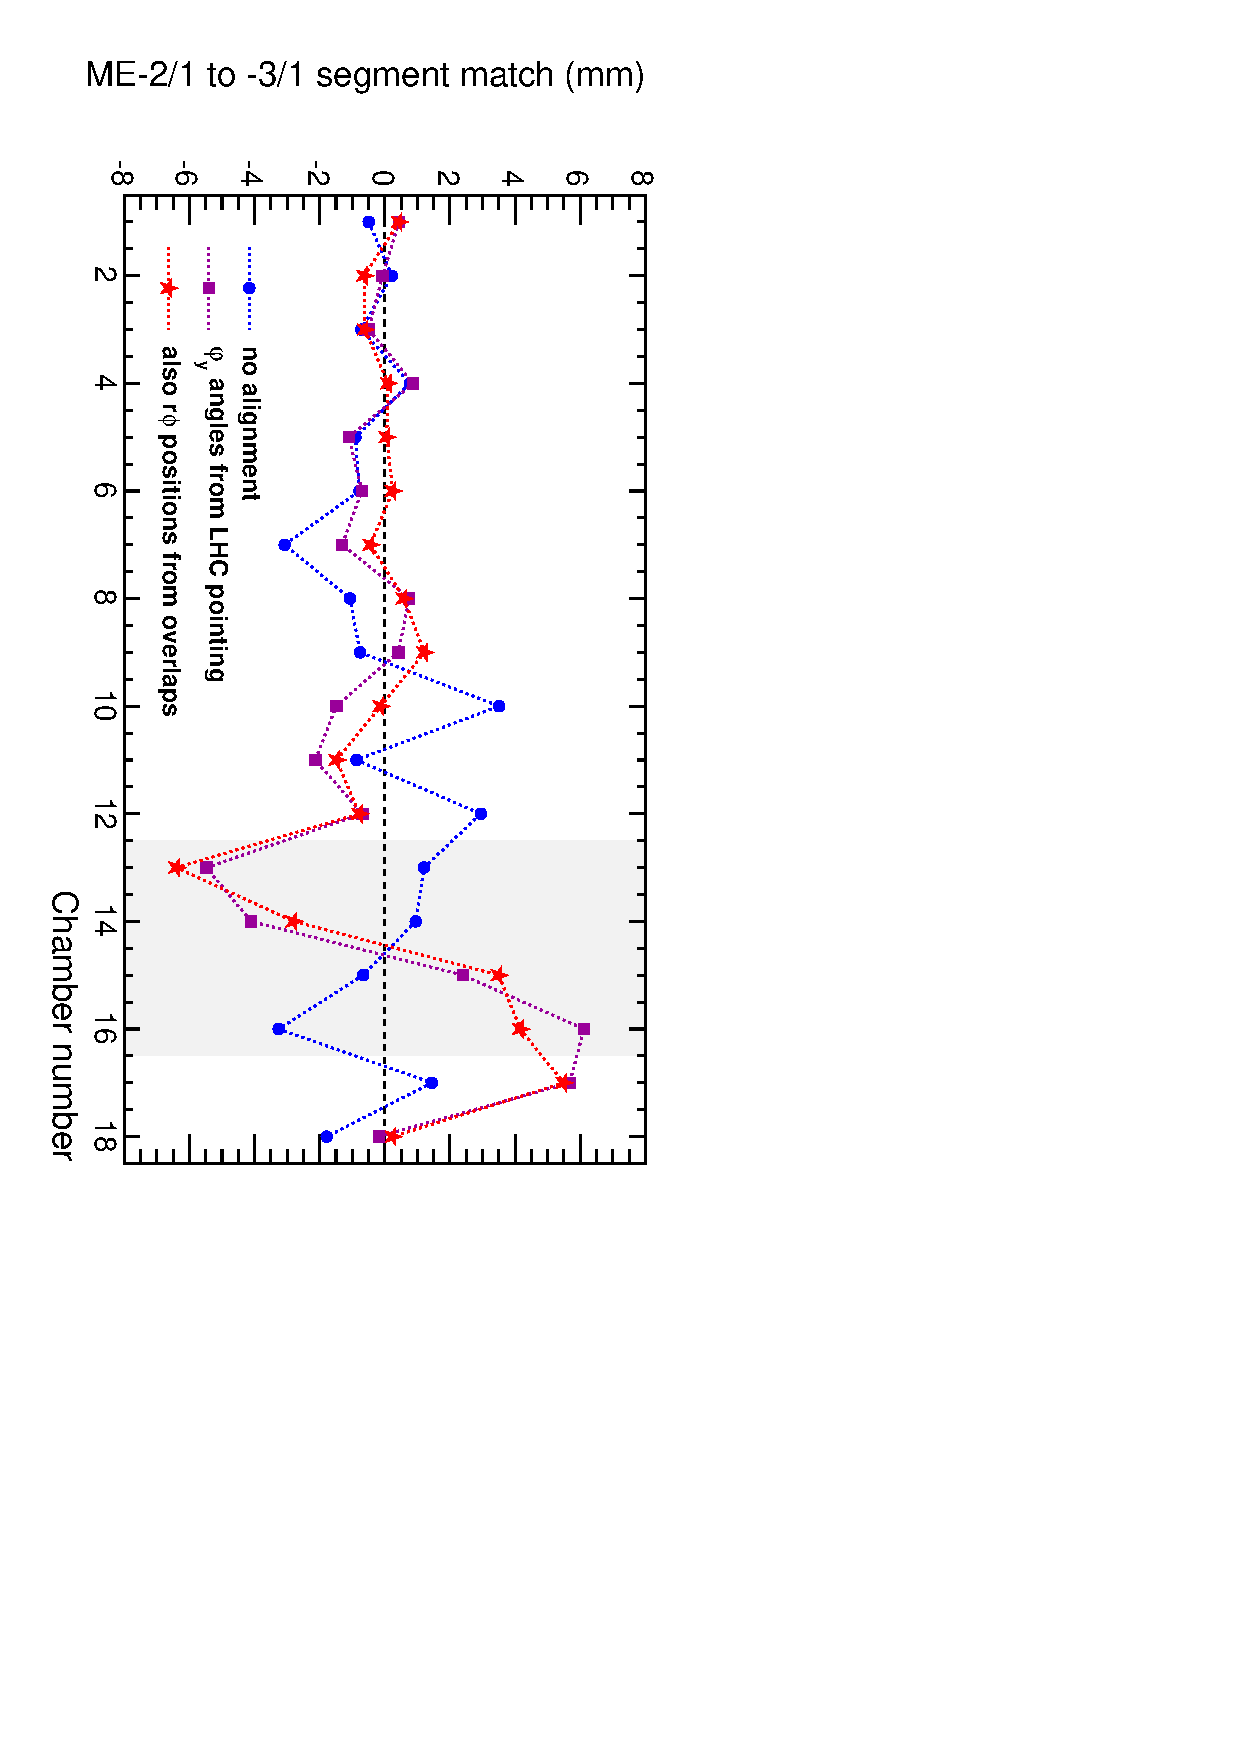
\includegraphics[height=0.75\linewidth, angle=90]{track_matching_better.pdf}}
\only<2>{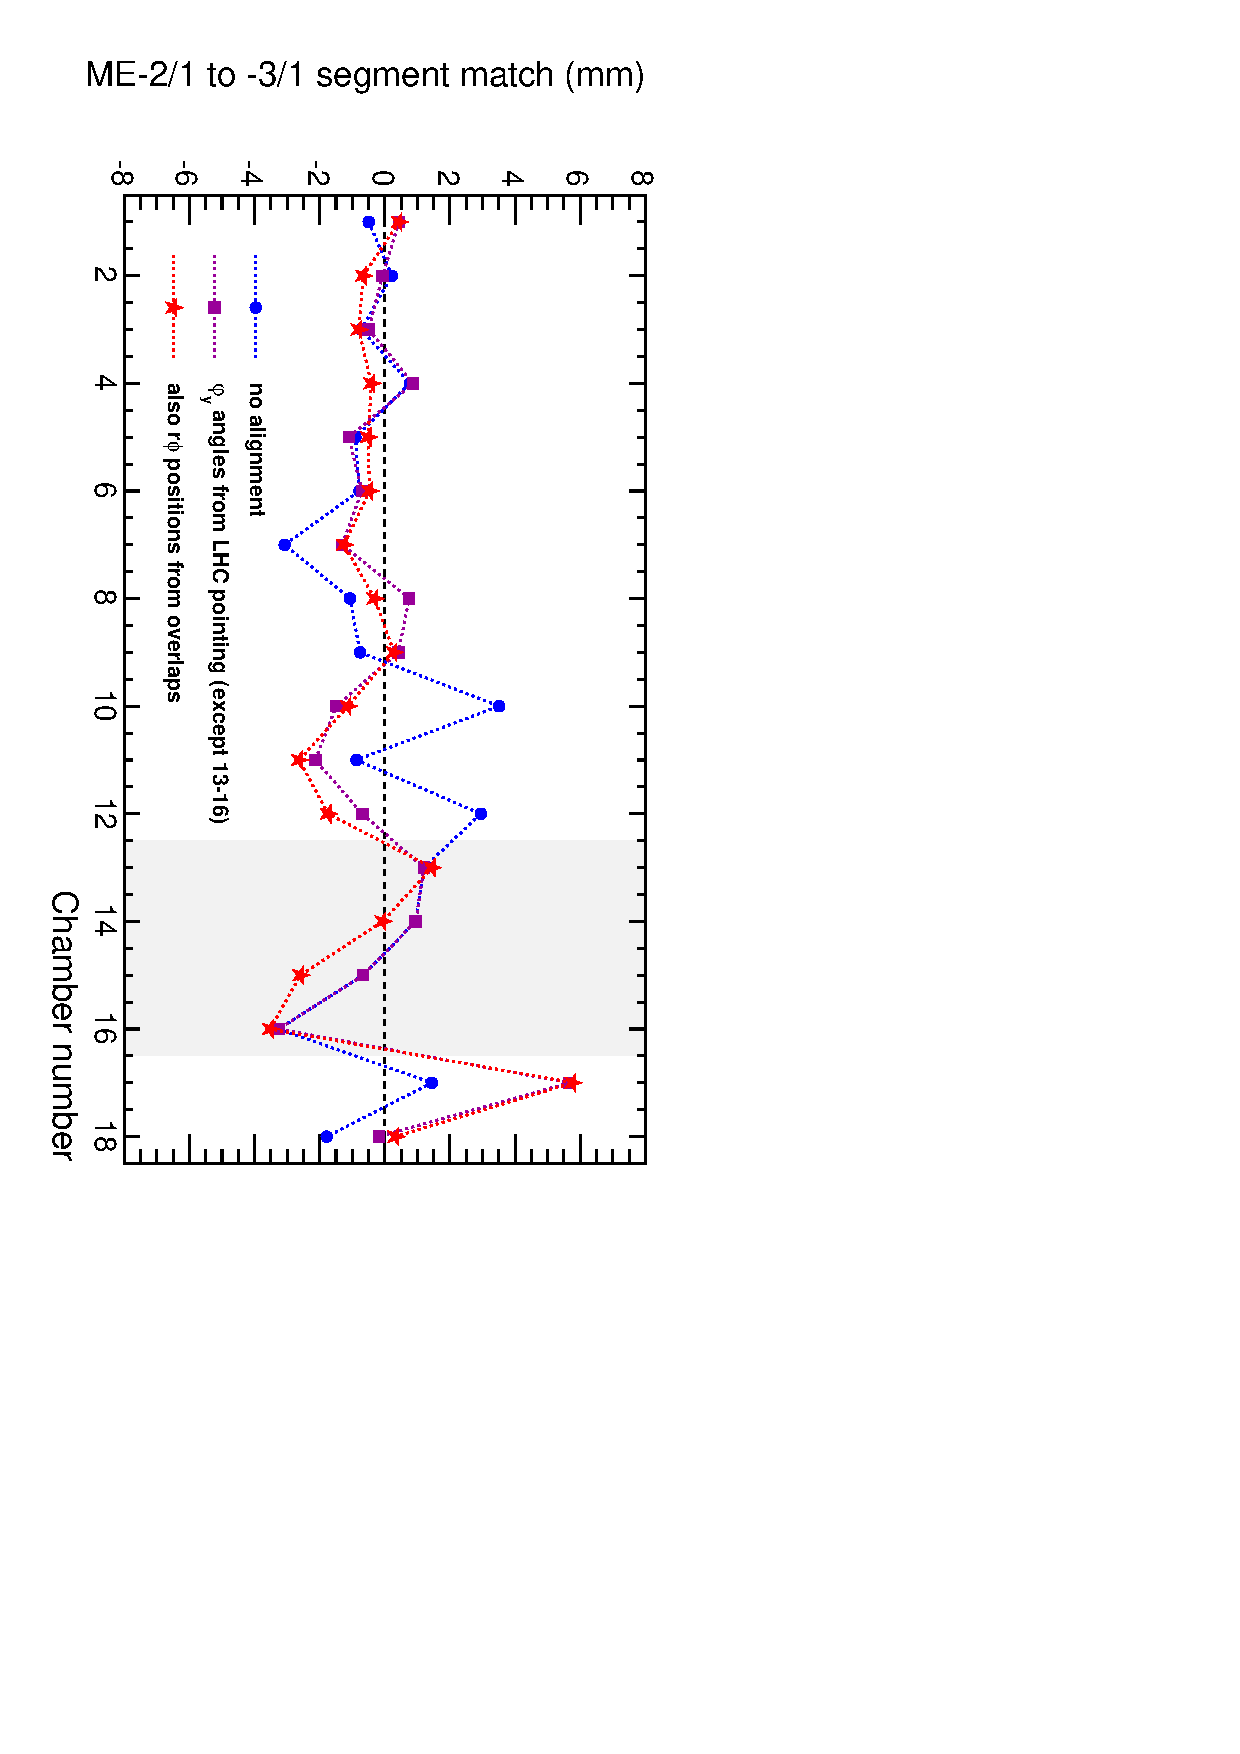
\includegraphics[height=0.75\linewidth, angle=90]{track_matching_better2.pdf}}

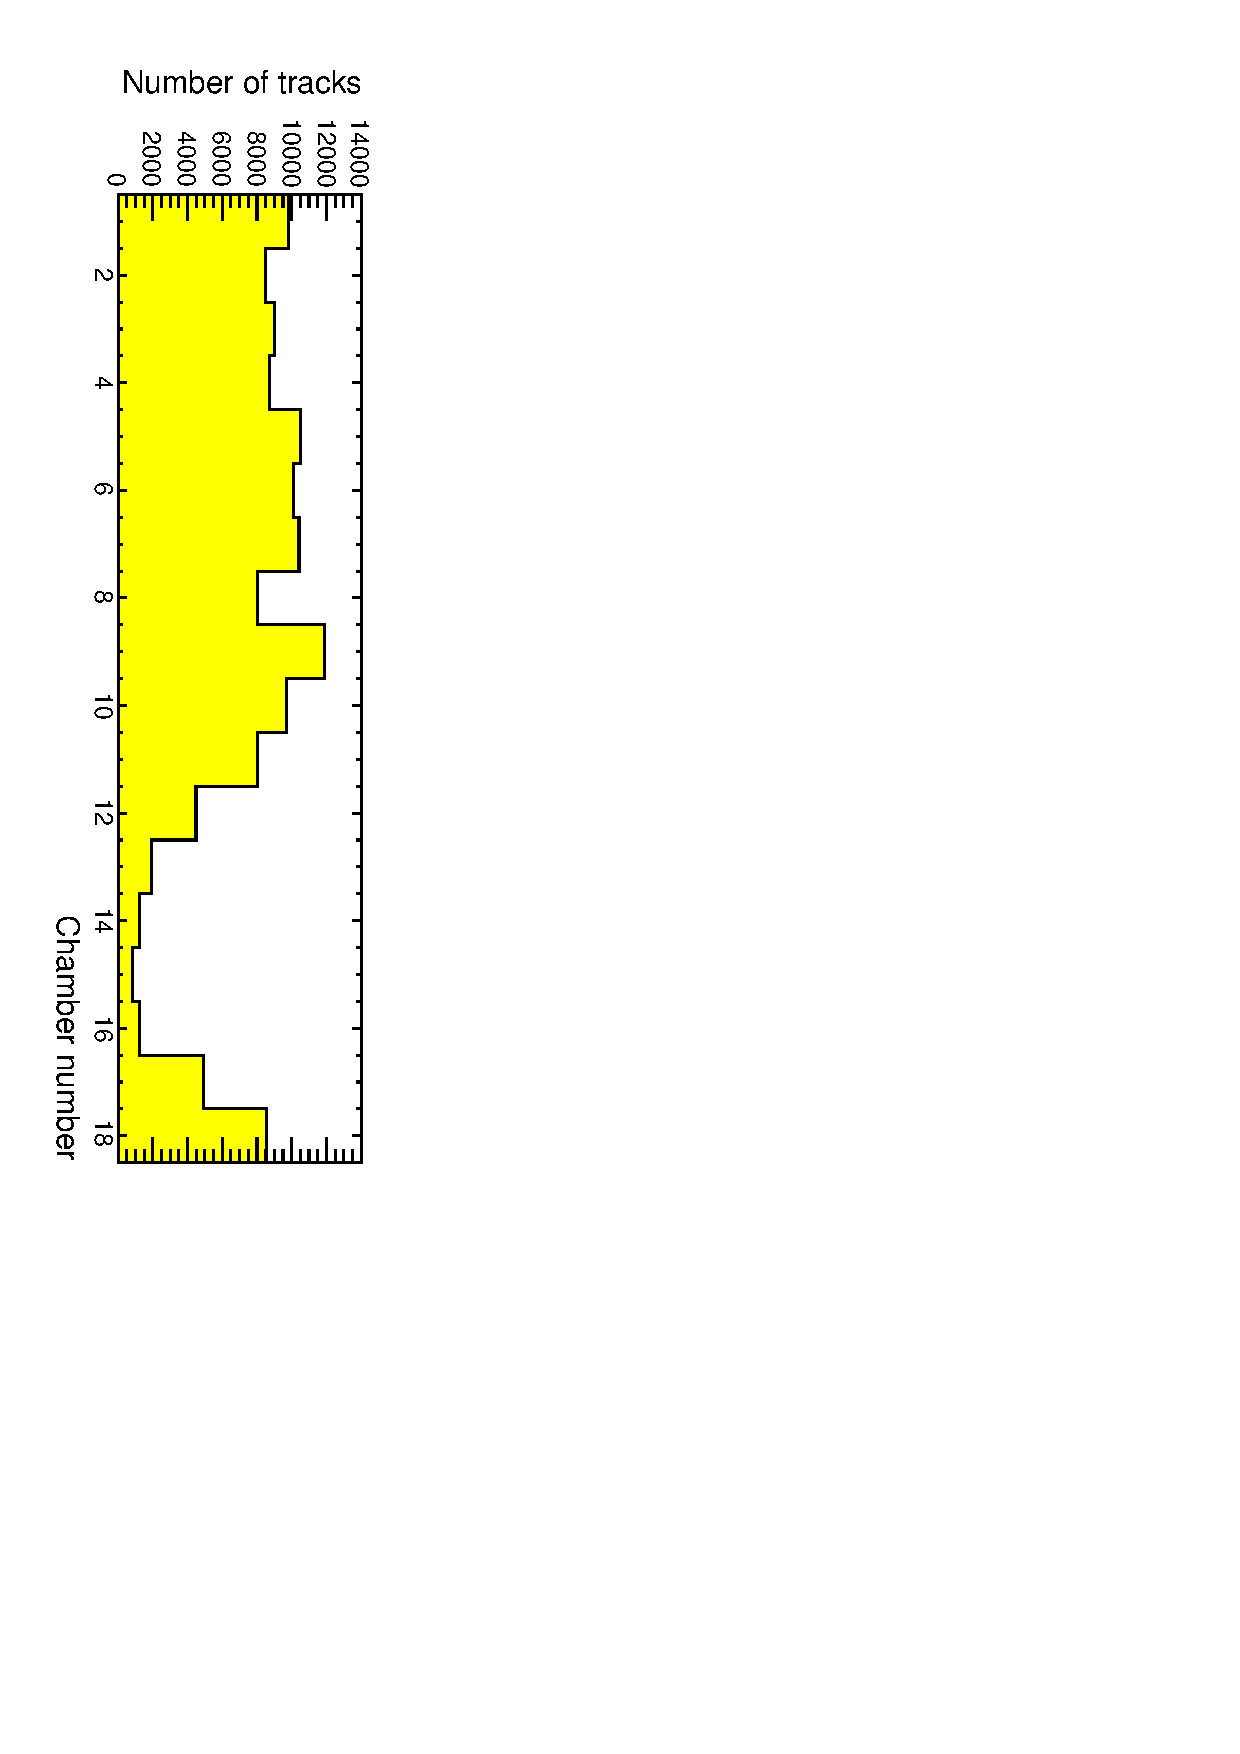
\includegraphics[height=0.75\linewidth, angle=90]{statistics.pdf}
\end{center}
\end{frame}

\begin{frame}
\frametitle{Diagnostic tool: 2-station fit}
\small

\begin{itemize}
\item Overlaps and straight-through tracks form a rigid frame: if errors are
not correlated between the rings, a combined fit would isolate errors
to one chamber (single-ring fit tries to distribute error uniformly)
\item Two benefits:
\begin{itemize}
\item diagnostic tool for identifying which chambers don't fit
\item yields the best set of constants with our present knowledge (excluding outliers)
\end{itemize}
\item But lose an independent cross-check
\end{itemize}

\vfill
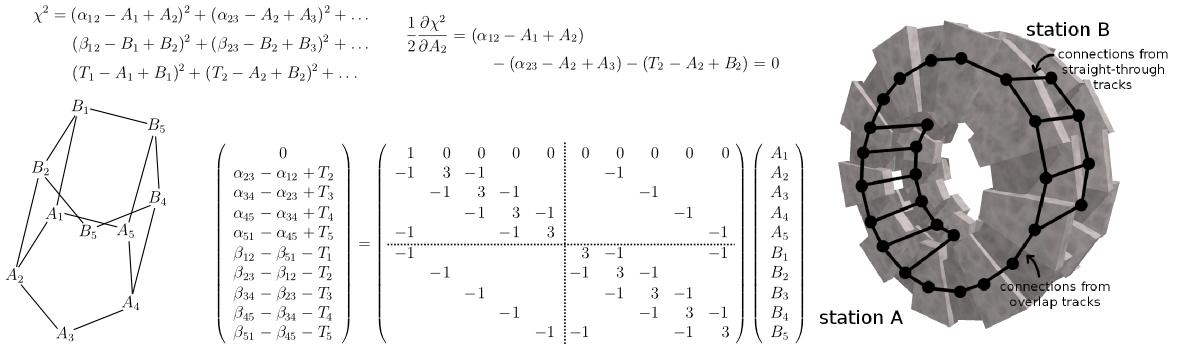
\includegraphics[width=\linewidth]{matrix_description.png}
\end{frame}

\begin{frame}
\frametitle{Example diagnostic}
\small

\vspace{0.5 cm}
\hspace{-0.5 cm} Overlap residuals from combined fit (red line is single-ring fit, \mbox{grey is unaligned)\hspace{-1 cm}}

\vfill
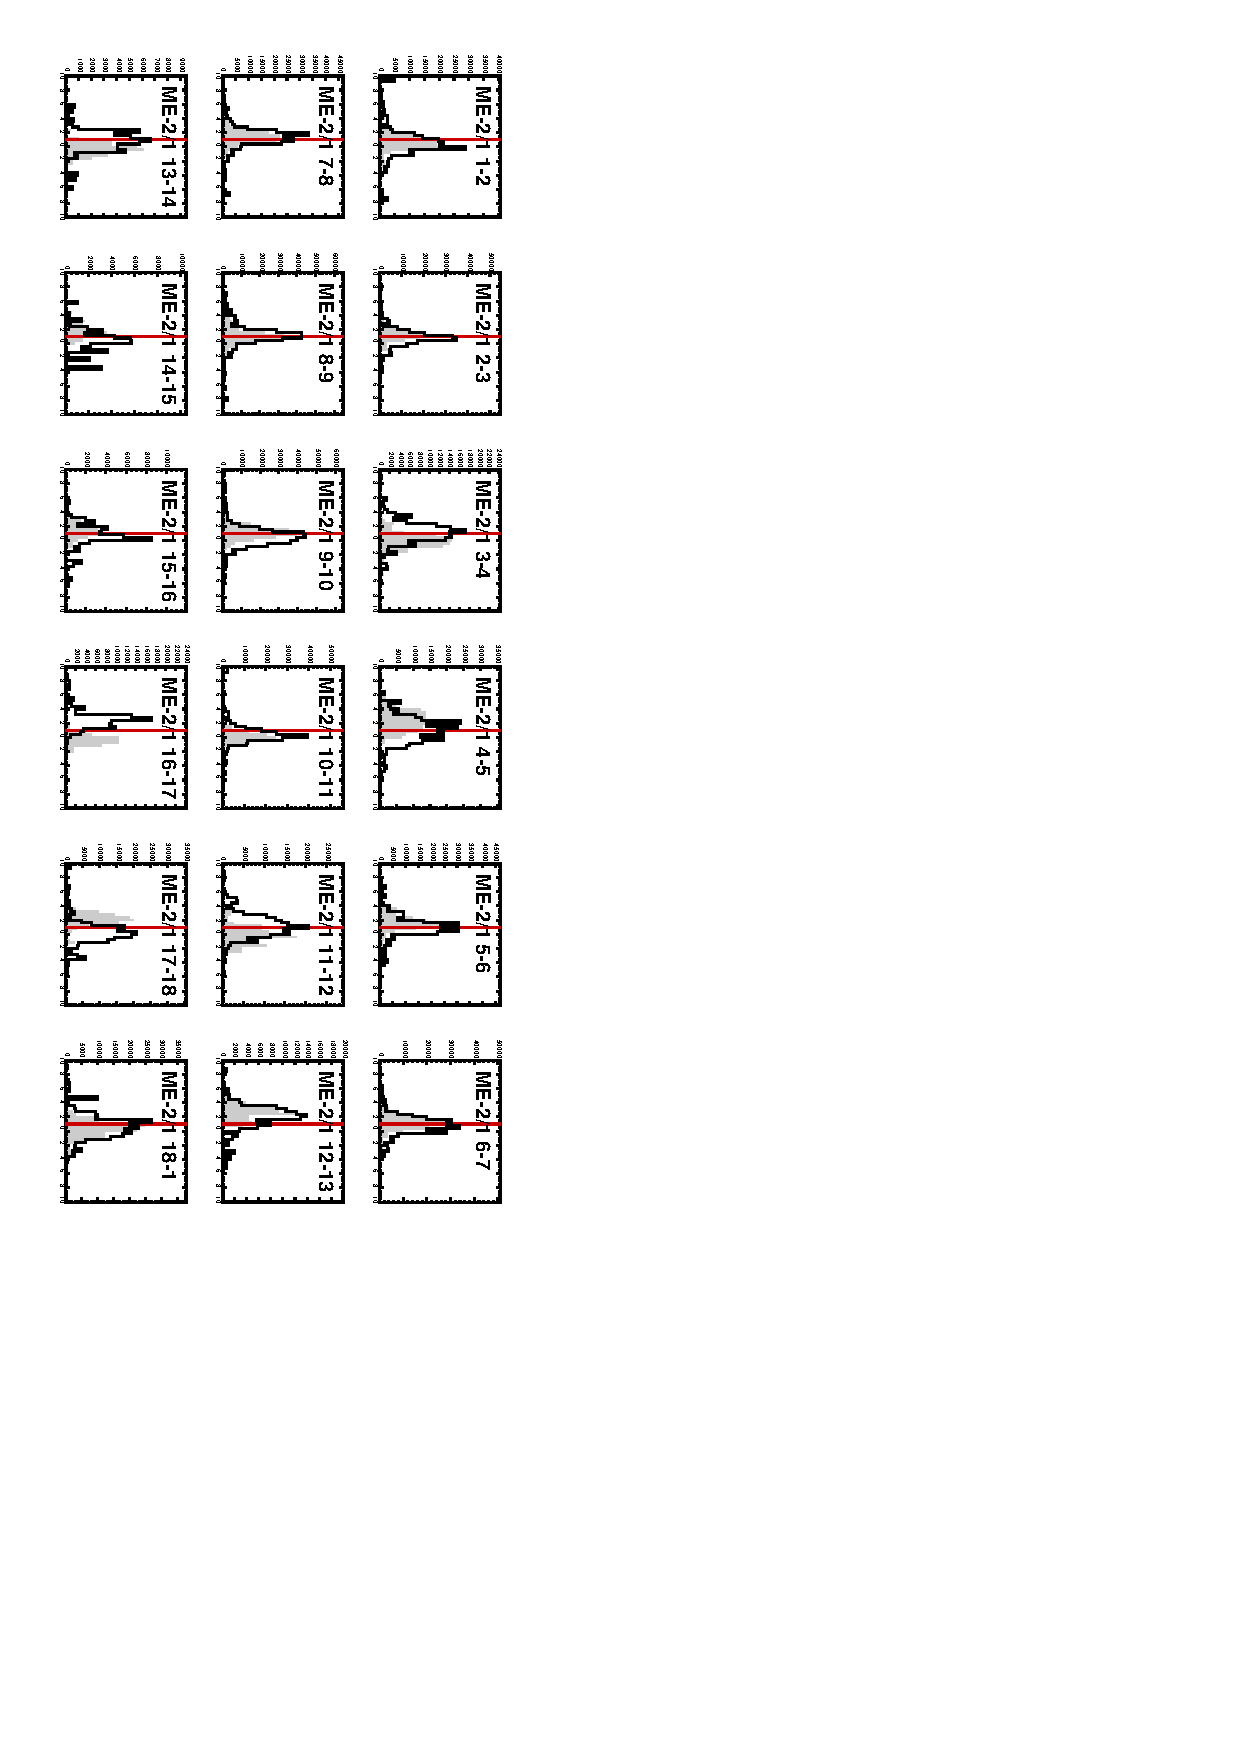
\includegraphics[height=\linewidth, angle=90]{final_checkresids_half.pdf}

\vfill
\begin{itemize}
\item Chamber 17 is clearly wrong (as we could have guessed from slide 10), also in ME$-$3/1, likely also a bad $\varphi_y$ angle
\item Single-ring fit would have made all final residuals equal

\vspace{0.5 cm}
\item Wide residuals from unaligned $\varphi_z$
\end{itemize}
\end{frame}

\begin{frame}
\frametitle{Current best results}
\small
\begin{itemize}
\item Constants from combined fit with chambers 13--16 unrotated
\item Chamber 17 has the wrong angle in either ME$-$2/1 or ME$-$3/1
\item Chambers marked ``questionable'' also don't fit well
\item $\infty$-stats Monte Carlo resolution is 2.2~mrad in $\varphi_y$, 0.37~mm in $r\phi$
\end{itemize}

\begin{center}
\only<1>{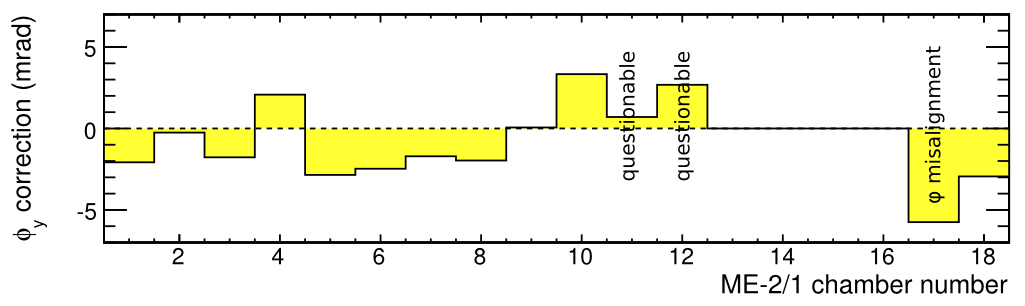
\includegraphics[width=0.9\linewidth]{present21_phiy.png}}
\only<2>{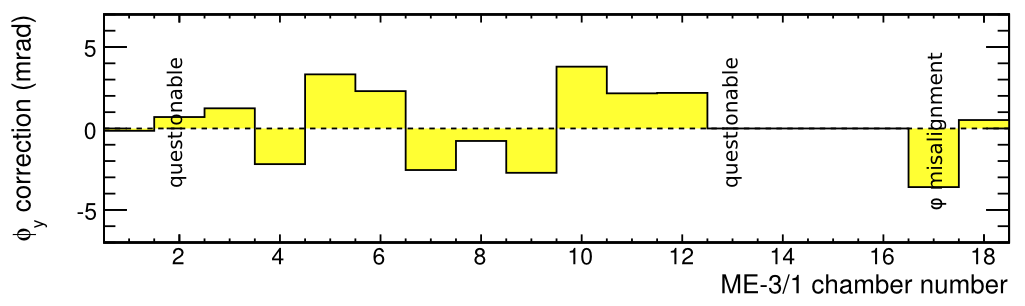
\includegraphics[width=0.9\linewidth]{present31_phiy.png}}

\only<1>{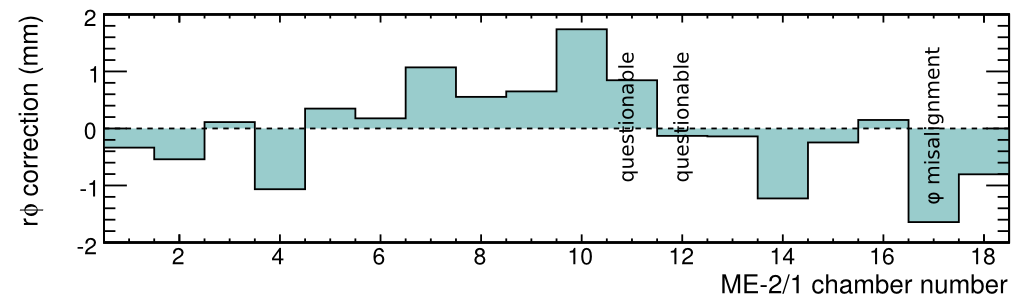
\includegraphics[width=0.9\linewidth]{present21_rphi.png}}
\only<2>{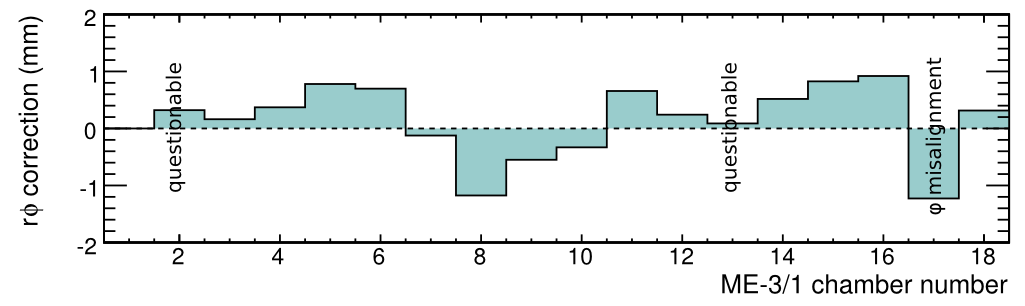
\includegraphics[width=0.9\linewidth]{present31_rphi.png}}
\end{center}
\end{frame}

\begin{frame}
\frametitle{Conclusions}

\begin{itemize}\setlength{\itemsep}{0.35 cm}
\item CSC Overlaps project has evolved into a special-purpose tool,
  but integrated into framework

\item Algorithm is correct: Monte Carlo alignment is perfect

\item Not all constraints satisfied in data: indication of unsimulated
  effects to discover in detector.  Diagnosing with cross-checks

\item However, current best constants have an RMS of 750~$\mu$m
  ($r\phi$) and 2.5~mrad ($\varphi_y$), indicating that random error
  in physical CSC placement and track-based alignment are both small

\item Comparison with hardware alignment in progress

\item Will be important for CRAFT because cosmic rays through both tracker
  and muon endcaps are scarce, magnetic field should be cross-checked
\end{itemize}

\label{numpages}
\end{frame}

\begin{frame}
\frametitle{Evolution of Overlaps Procedure}
\small
\begin{itemize}
  \item Plan in February: HIP iterations, alternating even and odd chambers
  \item Given few observables, reduced to 1D (local $x$) for better control
  \item Switched from full tracker to linear fits, again for better control
  \item Discovered a weak mode due to cancellation between left and
    right side of chamber; dropped hits from one side (used other side
    as cross-check)
  \item Removed discretization effects from wire granularity by
    parameterizing alignment in global $r\phi$, rather than local $x$
  \item Solve whole-ring alignment in one step to speed up convergence
  \item Algorithm works very well in Monte Carlo!  (accurate, ring closes)
  \item But in data, there were still some effects
\begin{itemize}
  \item Misalignment angles are significant, switched from a track fit
    on one side to track fits on both sides to be sensitive to
    relative angles
  \item Observe system with as many different data-driven methods as
    possible for confidence
\end{itemize}
\end{itemize}
\end{frame}





\end{document}
